\documentclass[letterpaper,12pt]{article}

\usepackage[utf8]{inputenc}
\usepackage[spanish,es-tabla]{babel}
\usepackage{graphicx}
\usepackage{amsmath,amssymb,amsfonts}
\usepackage{siunitx}
\usepackage{booktabs}
\usepackage{float}
\usepackage{caption}
\usepackage{hyperref}
\usepackage{fancyhdr}
\usepackage{ragged2e}
\setlength{\headheight}{14.5pt}
\usepackage{array}
\usepackage{xcolor}
\usepackage{multirow}
\usepackage{geometry}
\geometry{left=2.5cm, right=2.5cm, top=2.5cm, bottom=2.5cm}

\setlength{\parskip}{0.7em}
\setlength{\parindent}{0pt}
\allowdisplaybreaks[0]

\captionsetup{justification=justified}

\pagestyle{fancy}
\lhead{Sistema térmico TempControlLab}
\chead{2026-1}
\rhead{Universidad de Antioquia}
\cfoot{\thepage}

\graphicspath{{figures/}}

\begin{document}

\justifying

% ===================== PORTADA =====================

\begin{center}
\textsc{Universidad de Antioquia\\
Facultad de Ingeniería\\
Departamento de Ingeniería Electrónica\\
Sistemas de Control Continuo}

\vspace{1.2cm}


\includegraphics[height=2.5cm]{udea.png}

\vspace{0.8cm}

{\LARGE \textbf{TempControlLab UdeA: Sistema térmico con sensores LM35}}\\
{\large \textbf{Modelos de transferencia de calor aplicados}}

\vspace{1cm}

\textbf{Luis Alberto Ardila Páez}\\
\textbf{Daniel Esteban Tirado Rojas}\\
\textbf{Jose leonardo Perez Poveda}
\end{center}

\vspace{1cm}

\section{Introducción}

Este informe presenta la construcción y el modelado del sistema de control de temperatura \textit{TempControlLab UdeA}, utilizado en prácticas de laboratorio en la Universidad de Antioquia. La planta cuenta con dos calentadores (transistores de potencia) y dos sensores LM35, por lo que se trabaja con un sistema de dos entradas y dos salidas (MIMO).

Para describir su comportamiento, se parte de balances de energía expresados con ecuaciones diferenciales. En estas ecuaciones se incluyen los principales mecanismos de transferencia de calor: convección con el ambiente, conducción entre elementos y radiación entre superficies, además del efecto de inercia en la medición de los sensores.

Con este modelo físico y con los datos obtenidos en pruebas de escalón, se identifican modelos tipo \textit{First Order Plus Dead Time} (FOPDT). Estos modelos sirven como base para analizar la dinámica térmica y, en una etapa posterior, diseñar estrategias de control de temperatura.


\section{Propósito del laboratorio}

El propósito principal de este laboratorio es identificar experimentalmente un proceso térmico usando el sistema TempControlLab. Para ello, se aplican pruebas de escalón a los calentadores y se registran las respuestas de temperatura.

Con los datos obtenidos, se busca encontrar modelos dinámicos que relacionen las entradas del sistema (potencia en los calentadores) con las salidas (temperaturas medidas por los sensores). En particular, se ajustan modelos tipo \textit{First Order Plus Dead Time} (FOPDT), por ser una forma práctica y común de representar este tipo de procesos.

De manera específica, los objetivos del laboratorio son:

\begin{itemize}
\item Analizar la dinámica térmica del sistema experimental TempControlLab.
\item Obtener datos experimentales mediante pruebas de escalón en los calentadores.
\item Identificar modelos dinámicos del proceso utilizando distintos métodos de identificación.
\item Comparar los resultados obtenidos mediante los métodos de Ziegler–Nichols, Smith y optimización.
\item Analizar la interacción entre las variables del sistema, evidenciando el comportamiento MIMO del proceso térmico.
\end{itemize}


\section{Modelo físico del sistema}

El sistema TempControlLab funciona a partir de la transferencia de calor generada por resistencias eléctricas controladas con señales PWM desde una tarjeta Arduino. Cada calentador entrega energía térmica de acuerdo con la potencia aplicada, lo que eleva la temperatura de la placa metálica donde está instalado.

La dinámica térmica se describe con un balance de energía que considera los distintos mecanismos de transferencia de calor presentes en el proceso. De forma general, el comportamiento de cada elemento puede representarse con una ecuación diferencial del tipo

\begin{equation}
m c_p \frac{dT}{dt} = Q_{in} - Q_{out}
\end{equation}

donde $m$ es la masa del elemento térmico, $c_p$ es el calor específico del material y $T$ es la temperatura del sistema.

En el caso particular del TempControlLab, los principales mecanismos de transferencia de calor son:

\begin{itemize}
\item \textbf{Convección:} intercambio de calor entre el sistema y el ambiente circundante.
\item \textbf{Radiación térmica:} transferencia de energía entre superficies a diferentes temperaturas.
\item \textbf{Conducción:} transferencia de calor entre las dos placas térmicas del sistema.
\end{itemize}

El balance de energía para cada calentador se puede escribir, de forma simplificada, como

\begin{equation}
m c_p \frac{dT_H}{dt} =
UA(T_{\infty}-T_H)
+ \epsilon \sigma A (T_{\infty}^4 - T_H^4)
+ Q_{C12}
+ Q_{R12}
+ \alpha Q
\end{equation}

donde $UA$ representa la transferencia por convección con el ambiente, $\epsilon \sigma A$ representa la radiación térmica, $Q_{C12}$ corresponde al flujo de calor por conducción entre calentadores y $Q_{R12}$ al intercambio radiativo entre superficies.

Además, los sensores de temperatura tienen su propia dinámica por inercia térmica, la cual puede modelarse como

\begin{equation}
\tau_s \frac{dT_C}{dt} = T_H - T_C
\end{equation}

donde $T_C$ es la temperatura medida por el sensor y $T_H$ es la temperatura real de la superficie calentada.

Debido a la interacción térmica entre ambos calentadores, el sistema presenta acoplamiento entre variables: un cambio en un calentador puede afectar las dos temperaturas medidas. Por esta razón, se modela como un sistema MIMO con dos entradas y dos salidas.


\section{Interpretación del modelo identificado}

A partir de los datos obtenidos en las pruebas de escalón, se identificaron modelos FOPDT para cada relación entrada-salida del sistema. En general, este modelo se expresa como

\begin{equation}
G(s) = \frac{K}{\tau s + 1} e^{-\theta s}
\end{equation}

donde $K$ es la ganancia del proceso, $\tau$ es la constante de tiempo y $\theta$ es el tiempo muerto.

\section*{Toma de datos}

A continuación, se presentan las gráficas de las señales registradas y fotografías del montaje experimental de la planta térmica.

\begin{figure}[h!]
    \centering
    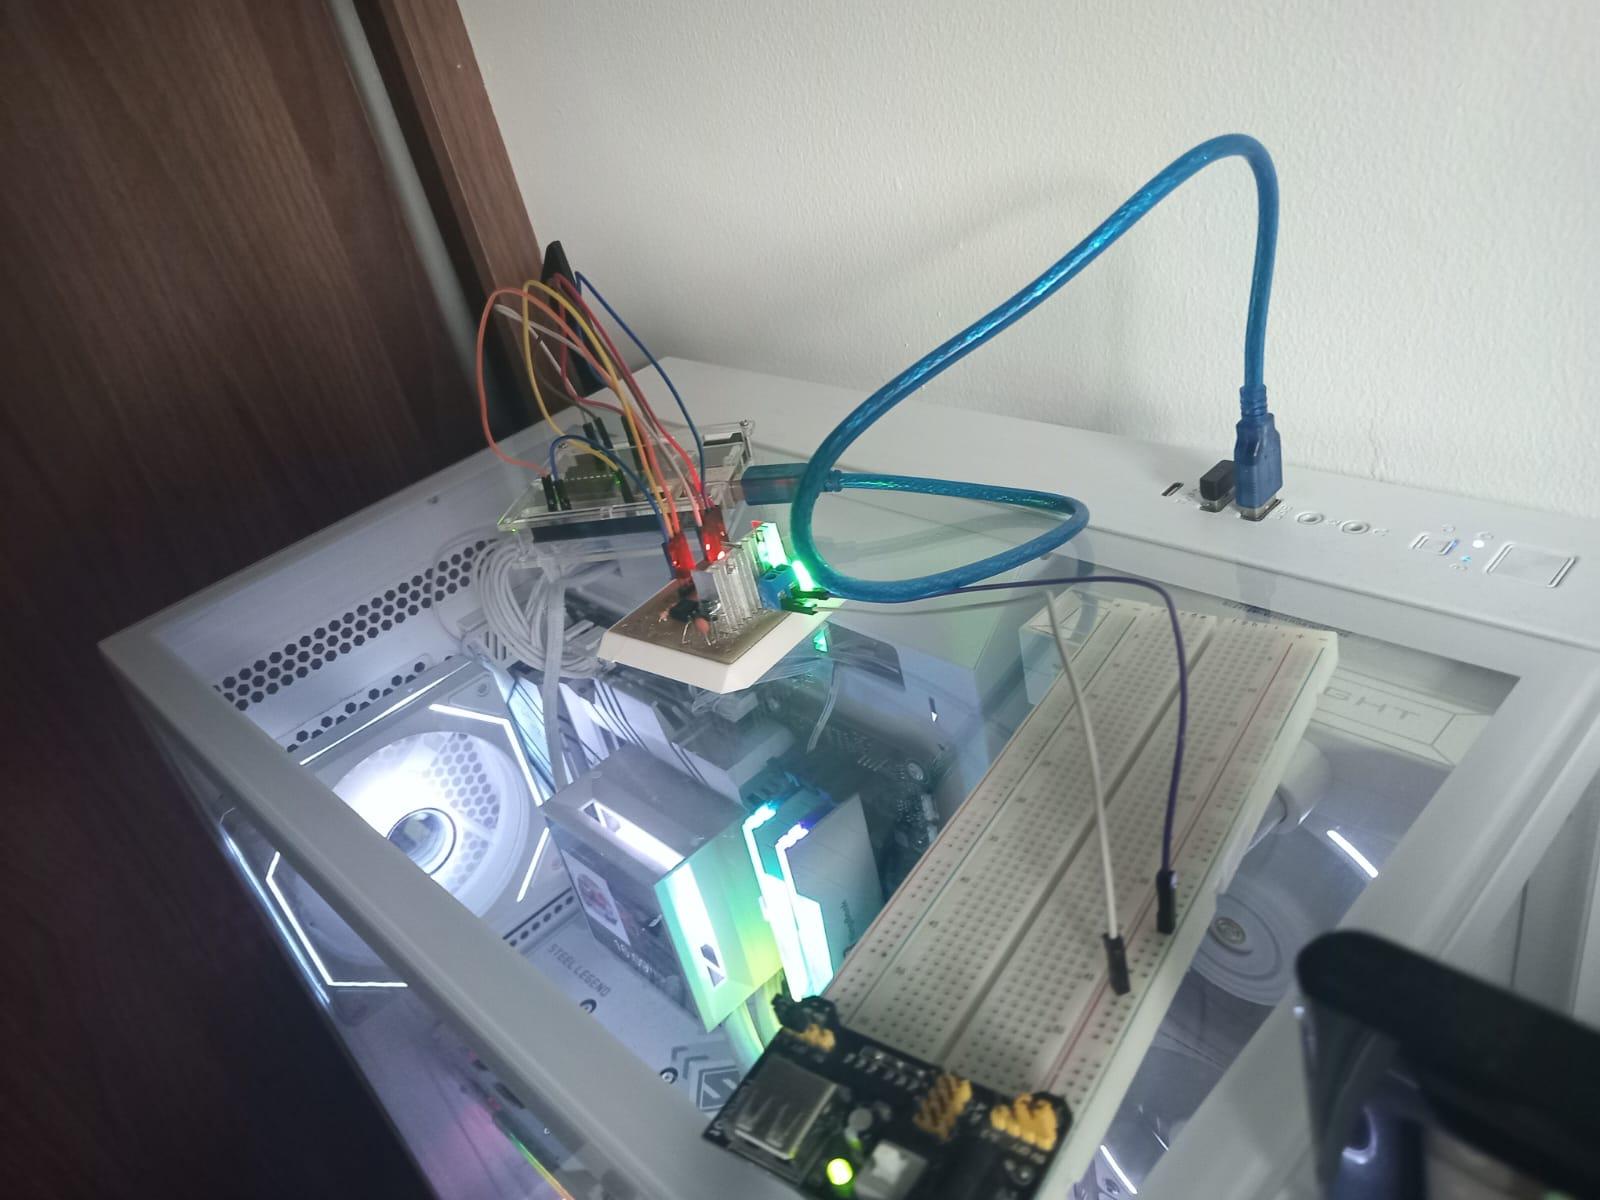
\includegraphics[width=0.45\textwidth]{imagen4.jpeg}
    \hfill
    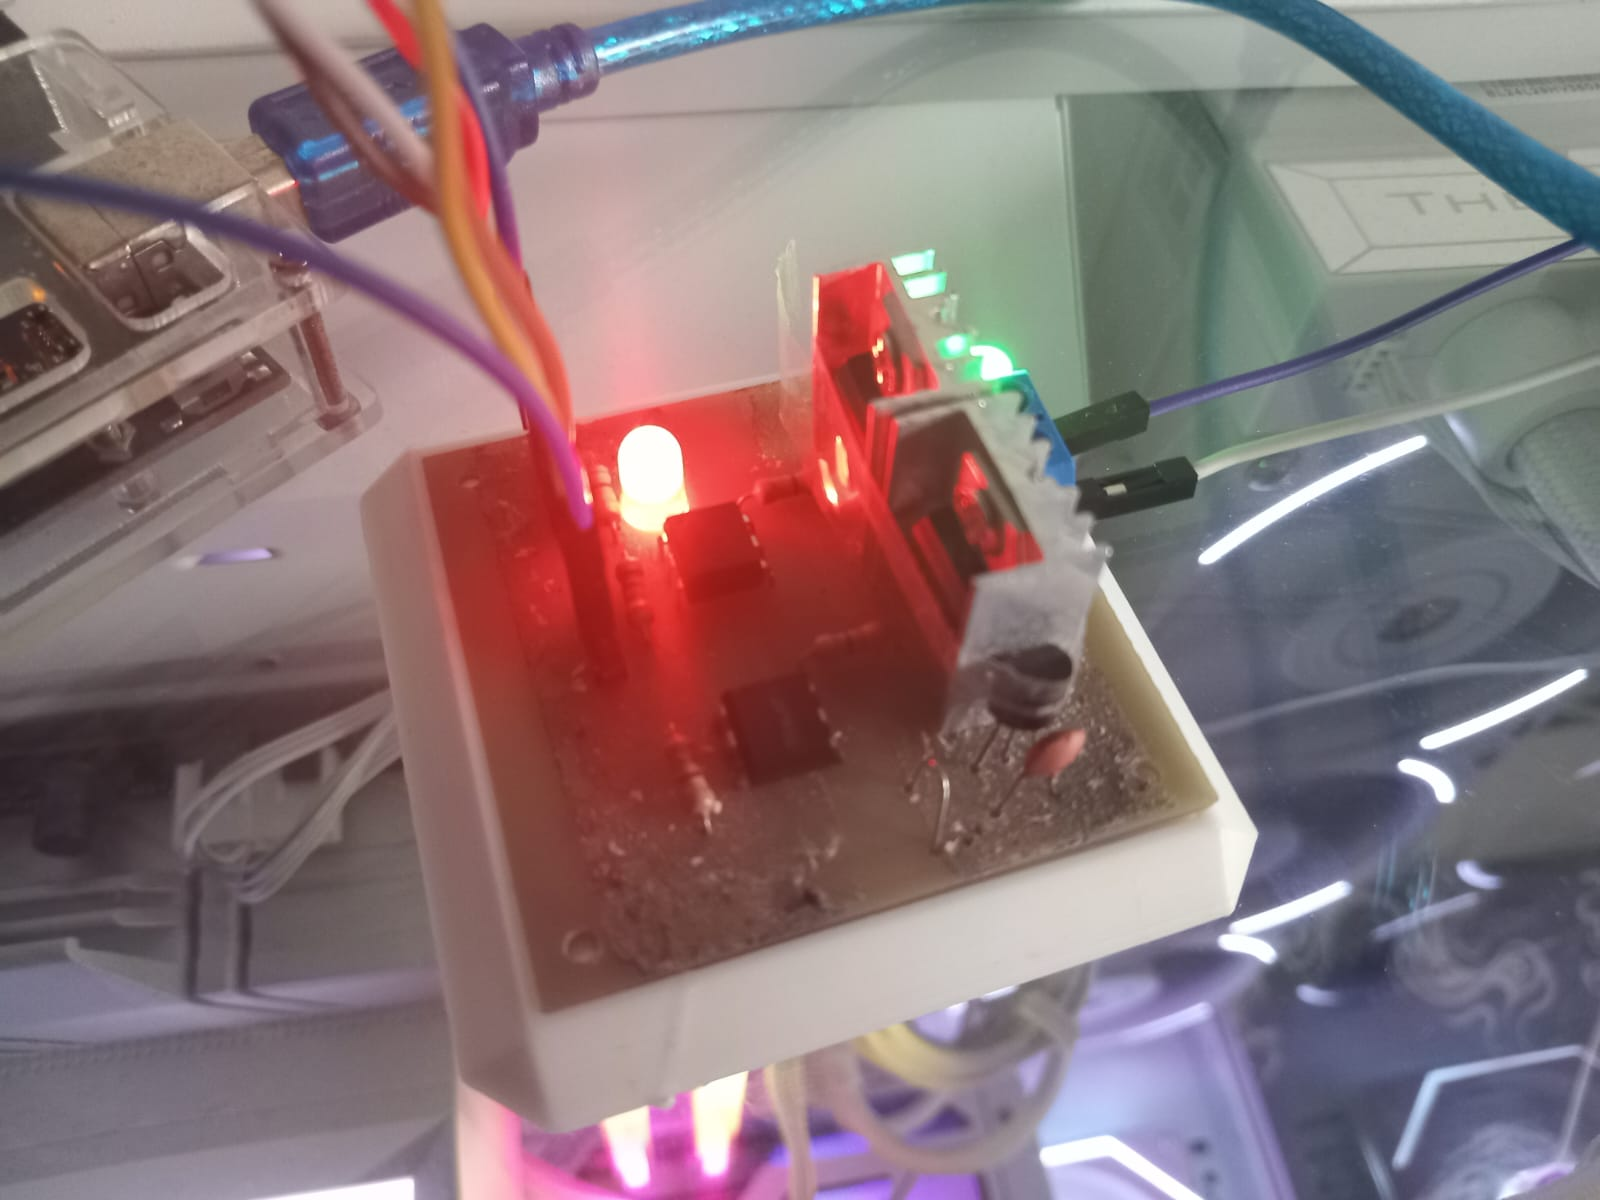
\includegraphics[width=0.45\textwidth]{imagen5.jpeg}
    \caption{Montaje físico de la planta térmica.}
\end{figure}

\begin{figure}[h!]
    \centering
    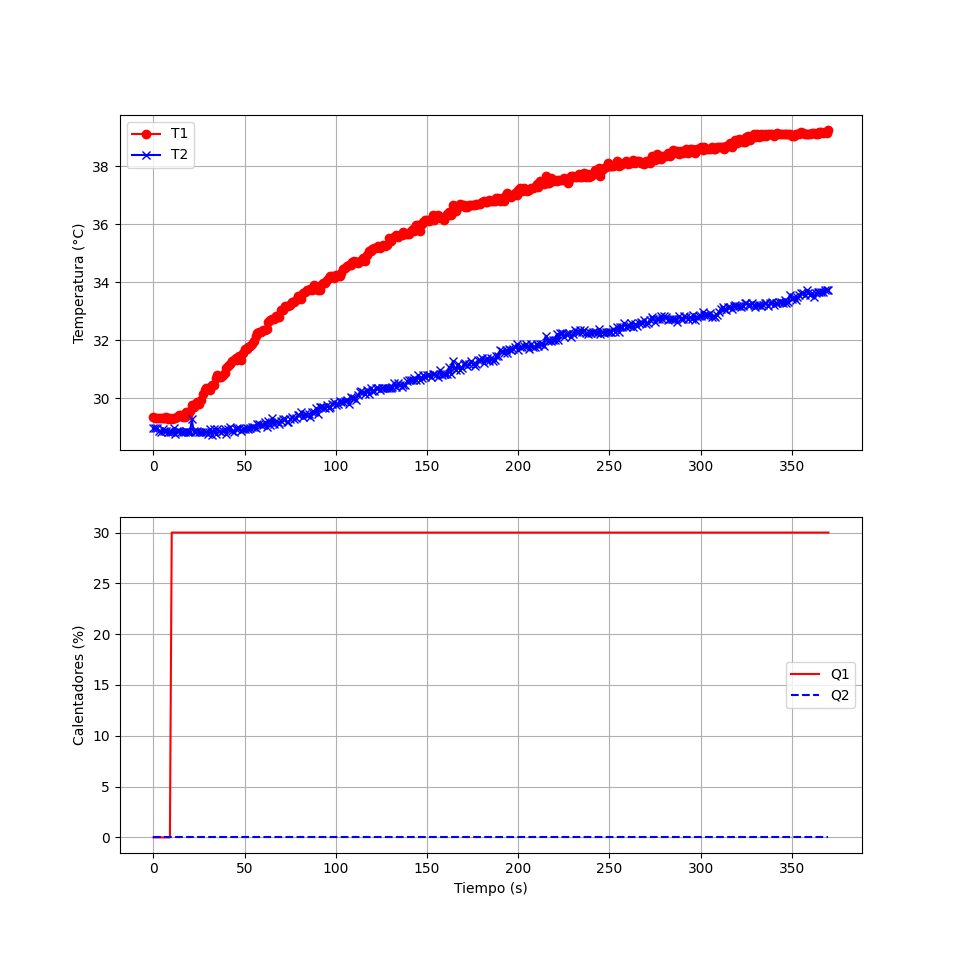
\includegraphics[width=0.45\textwidth]{UnicamenteQ1.png}
    \hfill
    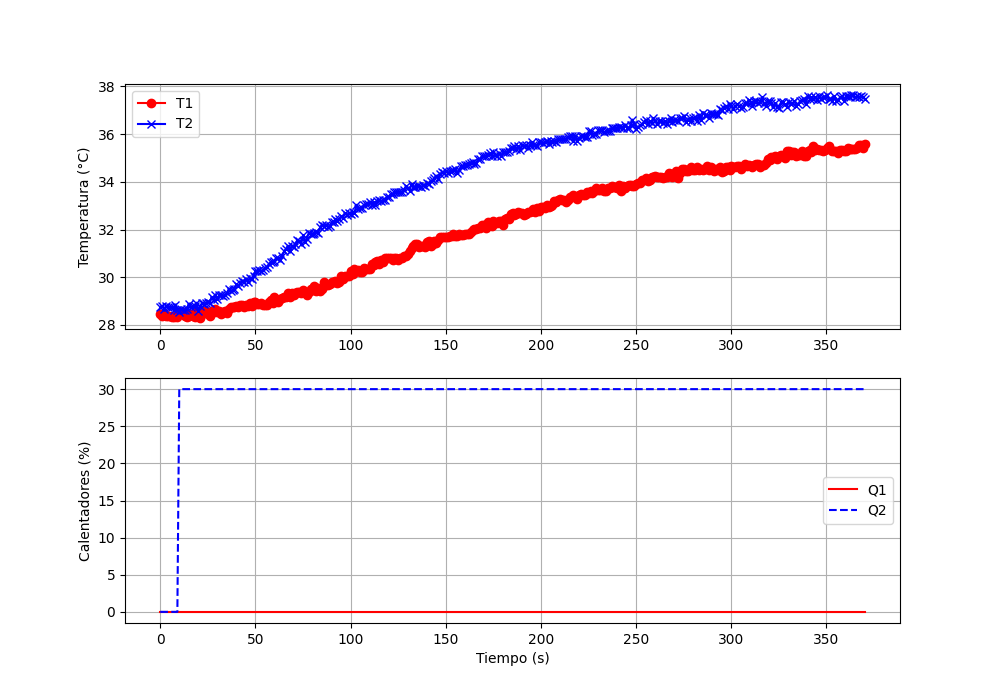
\includegraphics[width=0.45\textwidth]{UnicamenteQ2.png}
    \caption{Respuestas en lazo abierto con activación individual de Q1 o Q2.}
\end{figure}

\begin{figure}[h!]
    \centering
    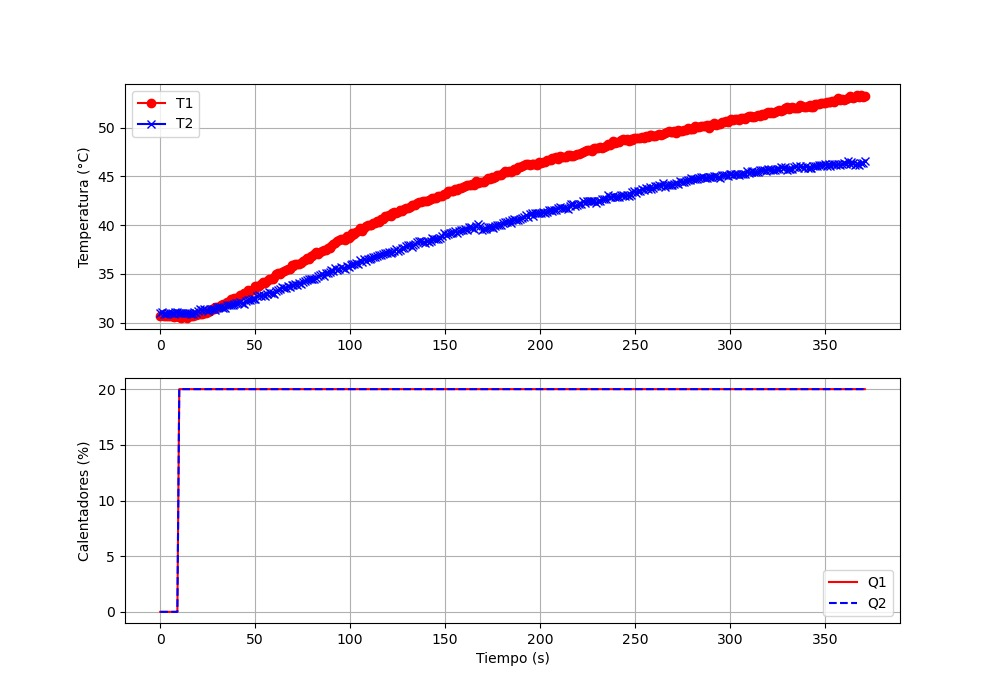
\includegraphics[width=0.45\textwidth]{imagen8.jpeg}
    \caption{Respuesta en lazo abierto con activación simultánea de Q1 y Q2.}
\end{figure}

\section*{Análisis del modelo FOPDT}

El modelo FOPDT se usa para describir sistemas con comportamiento de primer orden y retardo. En este análisis, se siguieron los pasos presentados a continuación para estimar los parámetros de ganancia \(K\), tiempo muerto \(\theta\) y constante de tiempo \(\tau\).

\subsection*{Pasos de identificación del modelo FOPDT}
\begin{enumerate}
    \item \textbf{Identificar el escalón de entrada:} Se analizó la señal de entrada para ubicar el instante en que inicia el cambio tipo escalón.
    
    \item \textbf{Ajustar el modelo FOPDT:} Se utilizó una regresión polinómica como referencia para describir la forma general de la respuesta térmica.
    
    \item \textbf{Aplicar los métodos de Ziegler-Nichols y Smith:} Se estimaron los parámetros del modelo a partir de la respuesta al escalón, obteniendo \(K\), \(\theta\) y \(\tau\).
    
    \item \textbf{Simular la respuesta al escalón con el modelo FOPDT:} Se usó la función de transferencia para reproducir la respuesta del sistema considerando el tiempo muerto.
    
    \item \textbf{Comparar los resultados:} Se compararon la respuesta real, la regresión polinómica y la respuesta simulada con el modelo FOPDT.
\end{enumerate}

\subsection*{Resultados}

Se desarrolló un código en un notebook de Jupyter para calcular los parámetros de los modelos a partir de los datos experimentales de la planta térmica, empleando las herramientas proporcionadas por TCLab. A continuación, se presentan los resultados obtenidos para el calentador Q1 mediante los métodos de Ziegler-Nichols y Smith:

\begin{itemize}
    \textbf{Ziegler-Nichols}
    \item \textbf{Ganancia:} \( K = 0.2931 \)
    \item \textbf{Tiempo muerto:} \( \theta = 12.5972 \, \text{segundos} \)
    \item \textbf{Constante de tiempo:} \( \tau = 169.0156 \, \text{segundos} \)
\end{itemize}

\begin{itemize}
    \textbf{Smith}
    \item \textbf{Ganancia:} \( K = 0.293 \)
    \item \textbf{Tiempo muerto:} \( \theta = 23.4411 \, \text{segundos} \)
    \item \textbf{Constante de tiempo:} \( \tau = 111.0140 \, \text{segundos} \)
\end{itemize}


\section*{Modelo para el calentador 1}

Se presentan las gráficas de comparación entre los métodos de Smith y Ziegler-Nichols, junto con la regresión polinómica ajustada.

\begin{figure}[h!]
    \centering
    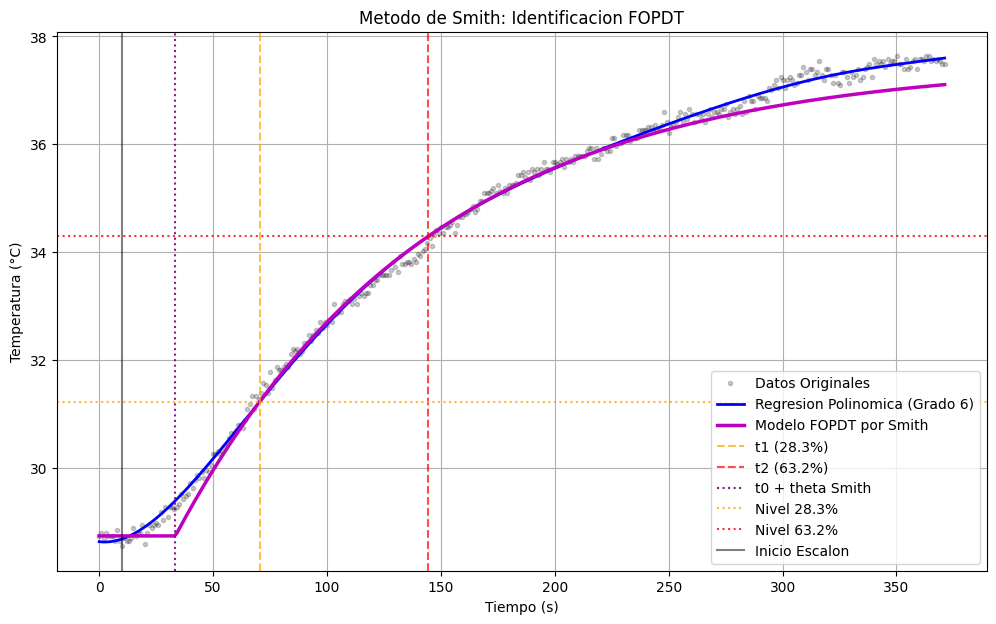
\includegraphics[width=0.45\textwidth]{grafica_smith.png}
    \hfill
    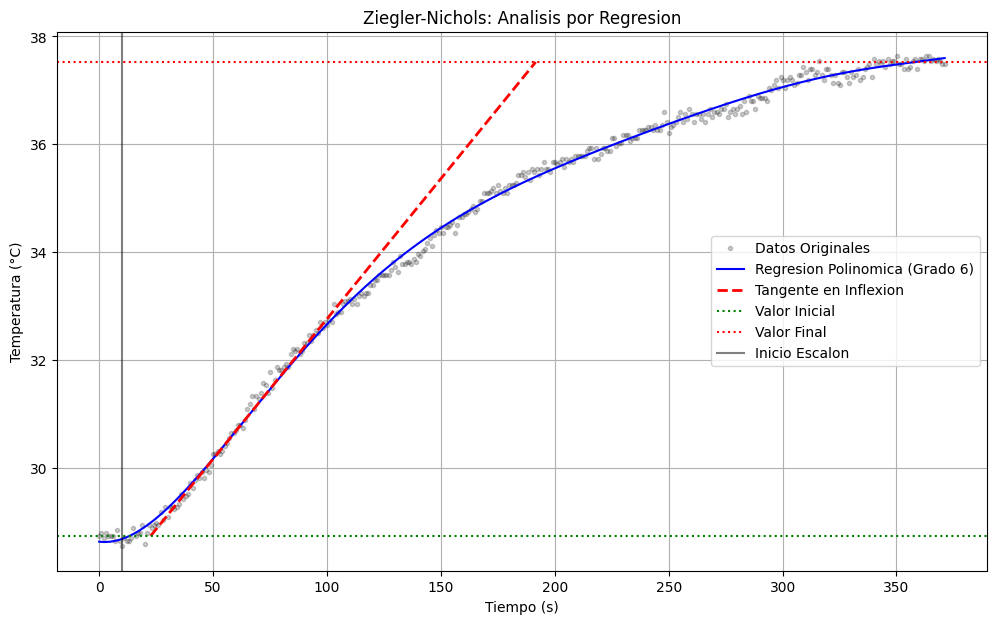
\includegraphics[width=0.45\textwidth]{grafica_nicolson.png}
    \caption{Comparación de respuestas para Q1: Smith (izquierda) y Ziegler-Nichols (derecha).}
\end{figure}

\begin{figure}[h!]
    \centering
    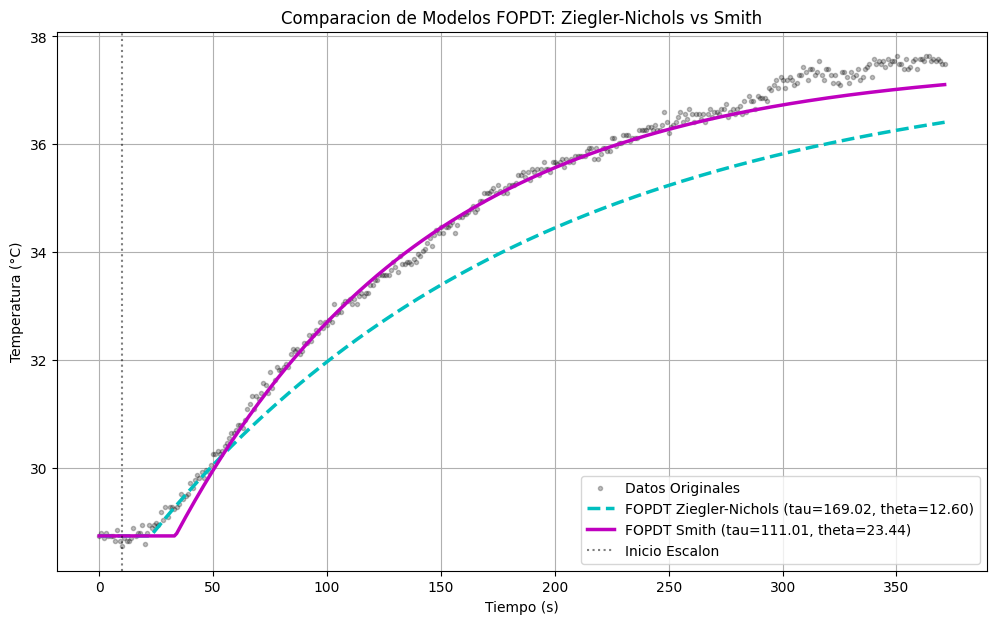
\includegraphics[width=0.7\textwidth]{compa.png}
    \hfill
    \caption{Comparación global de las respuestas para Q1.}
\end{figure}

\section*{Modelo para el calentador 2}

De manera análoga a lo realizado para Q1, se sigue el mismo procedimiento para estimar la función de transferencia del calentador 2 a partir de los datos experimentales de las pruebas de escalón.

% ===================== ESPACIO PARA IMÁGENES =====================
\begin{figure}[h!]
    \centering
    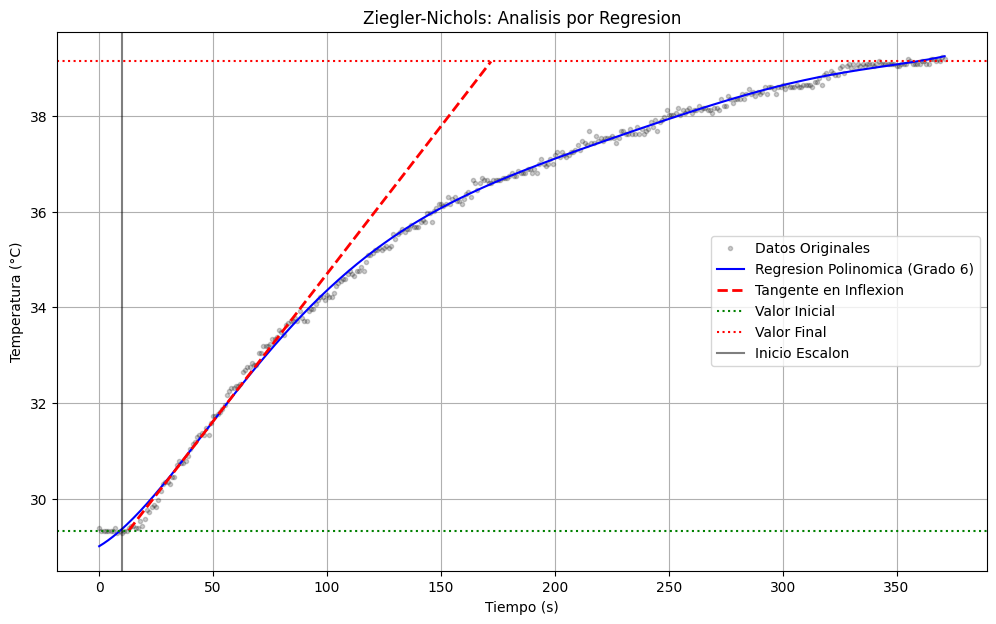
\includegraphics[width=0.45\textwidth]{imagen1.png}
    \hfill
    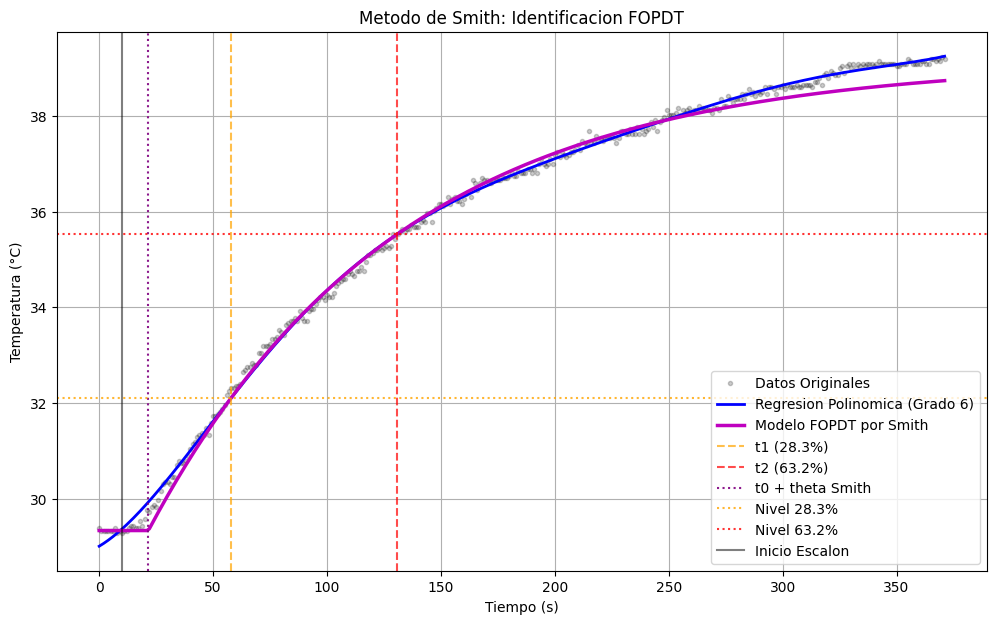
\includegraphics[width=0.45\textwidth]{imagen2.png}
    \caption{Comparación de respuestas para Q2.}
\end{figure}

\begin{figure}[h!]
    \centering
    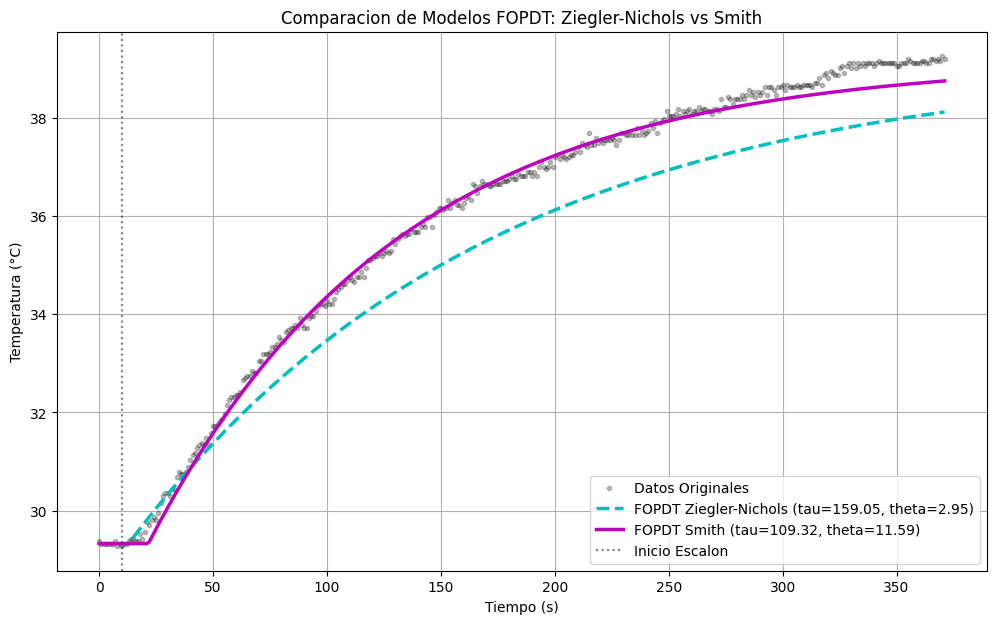
\includegraphics[width=0.7\textwidth]{imagen3.png}
    \caption{Respuesta simulada para Q2.}
\end{figure}

\section*{Conclusiones}

A partir de la comparación de los modelos FOPDT obtenidos con los métodos de Ziegler-Nichols y Smith, se concluye lo siguiente:

\begin{itemize}
    \item Los modelos ajustados por Ziegler-Nichols y Smith representan de forma adecuada el comportamiento general observado en los datos experimentales.
    \item Para Q1, ambos métodos estimaron una ganancia prácticamente igual (\(K \approx 0.293\)); sin embargo, difieren en los parámetros dinámicos: Ziegler-Nichols obtuvo \(\theta = 12.5972\,\text{s}\) y \(\tau = 169.0156\,\text{s}\), mientras que Smith obtuvo \(\theta = 23.4411\,\text{s}\) y \(\tau = 111.0140\,\text{s}\).
    \item Estas diferencias muestran que cada método ajusta de manera distinta la respuesta al escalón, lo cual puede influir en los resultados de simulación y en el diseño del controlador.
    \item En la práctica, ambos modelos son útiles para una primera aproximación; sin embargo, la selección final debe validarse con criterios de error y pruebas en lazo cerrado.
\end{itemize}

En conclusión, los métodos de identificación utilizados permiten representar de forma adecuada el comportamiento del sistema térmico estudiado. Como trabajo futuro, se recomienda complementar la validación con métricas de ajuste (por ejemplo, IAE, ISE o RMSE) y evaluar el desempeño de controladores diseñados a partir de cada modelo.

\section*{Referencias}

\begin{enumerate}
    \item Alfaro, V. M. (2001). \textit{Identificación de procesos sobreamortiguados utilizando técnicas de lazo abierto}. Revista Ingeniería, 11(1--2), 11--25.
    
    \item TCLab Documentation. (consulta: 2026). \textit{Documentación oficial de TCLab}. \url{https://tclab.readthedocs.io/}
\end{enumerate}


\end{document}


